\documentclass{book}

\usepackage{ardour,graphicx,afterpage,url}

% XXX: format
\newcommand{\button}[1]{#1}
\newcommand{\menu}[1]{#1}

\newcommand{\screenshot}[3]{%
\begin{figure}[ht]%
\begin{center}
\includegraphics[scale=0.5]{screenshots/#1}
\end{center}
\caption{#2}
\label{#3}
\end{figure}}


\title{Ardour 3 --- A users' manual}
\author{The Ardour Community}
\date{}
\begin{document}

\maketitle

\tableofcontents

\chapter{Introduction}

Hello, and welcome to Ardour!

\section{What is Ardour?}

Ardour is an open-source digital audio workstation (DAW) for Linux and Mac OS~X.


\section{Typographical conventions}

This manual takes a cue from the \TeX{}book and uses special symbols
to denote sections which contain advanced material.  Readers can
skip these sections without any great loss.

\begin{danger}
Tricky parts of the text are marked with a `bend in the road' marker.
They contain extra information which may be of interest to advanced
users.
\end{danger}

\begin{ddanger}
Especially tricky parts of the text are marked with a double
bend-in-the-road marker.  Such sections will only be of interest to
the completist or serious hacker.
\end{ddanger}


\chapter{Overview}

As one might expect, Ardour is similar in many ways to many other DAWs
and also has its fair share of differences.  This chapter gives an
overview of Ardour.


\section{JACK}

Ardour is built on another piece of software called JACK\footnote{JACK
  stands for the JACK Audio Connection Kit; a pleasingly recursive acronym}.
JACK has two main functions; first, it moves audio and MIDI to
and from a sound card, and second, it allows audio and MIDI to be
routed between different applications.

JACK provides a great deal of flexibility and power, especially when
running other applications (such as soft-synthesizers or samplers) at
the same time as Ardour.  It is somewhat similar to Steinberg's Rewire
technology, though broader in scope.  It is even possible to use JACK
to route audio and MIDI over network connections.

JACK is so important to Ardour's operation that it earns its own
discussion in chapter~\ref{ch:jack}.


\section{Sessions}

An Ardour \emph{session} is a container for an entire project.  A
session may contain an arbitrary number of tracks and busses
consisting of audio and MIDI data, along with information on processing
those tracks, a mix of levels, and everything else related to the
project.  A session might typically contain a song, or perhaps an entire
album or a complete live recording.

Ardour sessions are held in directories; these directories contain one
or more \emph{session files}, some or all of the audio and MIDI data
and a number of other state files that Ardour requires.  The session
file describes the structure of the session, and holds automation data
and other details.

\begin{danger}
Ardour's session file is kept in XML format, which is advantageous as
it is somewhat human-readable, and human-editable in a crisis!  Sound
files are stored in one of a number of optional formats, and MIDI
files as SMF (standard MIDI format).

It is also possible for Ardour sessions to reference sound and MIDI
files outside the session directory.
\end{danger}

Ardour has a current session at all times; if Ardour is started without
specifying one, it will offer to load or create one.



\section{Tracks}

A track is a concept common to most DAWs, and used also in Ardour.
Tracks can record audio or MIDI data to disk, and then replay it with
processing.  They also allow the audio or MIDI data to be edited in a
variety of different ways.

In a typical pop production, one might use a track each for the kick
drum, another for the snare, more perhaps for the drum overheads and
others for bass, guitars and vocals.

Ardour can record to any number of tracks at one time, and then play
those tracks back.  On playback, a track's recordings may be processed
by any number of plugins, panned, and its level altered to achieve a
suitable mix.

\begin{danger}
A track's type is really only related to the type of data that it
stores on disk.  It is possible, for example, to have a MIDI track
with a synthesizer plugin which converts MIDI to audio.  Even though
the track remains `MIDI', in the sense that its on-disk recordings are
MIDI, its output may be audio-only.
\end{danger}


\section{Regions}

A track may contain many segments of audio or MIDI\@.  Ardour contains
these segments in things called \emph{regions}, which are
self-contained snippets of audio or MIDI data.  Any recording pass,
for example, generates a region on each track that is enabled for
recording.  Regions can be subjected to many editing operations; they
may be moved around, split, trimmed, copied, and so on.


\section{Playlists}

The details of what exactly each track should play back is described
by a \emph{playlist}.  A playlist is simply a list of regions; each
track always has an active playlist, and a track's current playlist
can always be changed.


\section{Busses}

Busses are another common concept in both DAWs and hardware mixers.
They are similar in many ways to tracks; they process audio or MIDI,
and can run processing plugins.  The only difference is that their
input is obtained from other tracks or busses, rather than from disk.

One might typically use a buss to collect together the outputs of
related tracks.  Consider, for example, a 3-track recording of a
drum-kit; given kick, snare and overhead tracks, it may be helpful to
connect the output of each to a bus called `drums', so that the
drum-kit's level can be set as a unit, and processing (such as
equalisation or compression) can be applied to the mix of all tracks.


\chapter{JACK}
\label{ch:jack}

\section{Introduction}

JACK is the JACK audio connection kit.  It is a piece of software that
provides the low-level `plumbing' which allows Ardour to work.  Its
setup is crucial to Ardour; Ardour will not work without it.

JACK's essential task is to route audio and MIDI data to and from a
sound card, and also between applications.  It manages a set of
\emph{ports}, which it can connect together in arbitrary ways.
Figure~\ref{fig:typical-jack-session} gives a diagram of a moderately
complex JACK session.

\begin{danger}
JACK is not limited to the standard concept of the `sound card'.  One
may choose to have no sound card at all (in which case JACK can run in
`dummy' mode).  It is also possible to send signals to and from JACK
over TCP/IP networks using netjack.  For simplicity, this manual will
assume that the user has a sound card in the conventional sense.
\end{danger}


\subsection{JACK versions}

For historical reasons, there are two `branches' of JACK that are both
maintained, and can be used as drop-in replacements for each other.
JACK1 has version numbers like 0.121.3, and JACK2 (also known as
jackdmp) has version numbers like 1.9.8.  Both implementations have
their advantages and disadvantages.  It does not matter a great deal
which one is used.

% XXX: unless what?


\section{Starting JACK}

Ardour can start JACK automatically when it starts; and indeed many
users will find that this works perfectly well.  It is also possible
to start JACK manually, either at the command line or using a tool
such as QJackCtl\footnote{\url{http://qjackctl.sourceforge.net}} or
JackPilot\footnote{\url{http://www.jackosx.com}}.

\subsection{Parameters}

JACK has many parameters which affect its operation.  Some of the more
important ones are discussed here.

\subsubsection{Sampling rate}

This is the number of samples per second that JACK will process, and
is important as it will govern the sampling rate that all audio
applications will run at.  The chosen rate must be supported
by the sound card, so values such as 44.1kHz, 48kHz, 96kHz
et.\ cetera are typical choices.  The higher the sampling rate, the
higher the theoretical audio frequency that the system can reproduce,
but also the more disk space will be consumed by audio recordings, and
the more CPU power will be required to run audio plugins.

\subsubsection{Frames per period}

In a move necessary for efficiency, JACK does not process audio
sample-by-sample, but in blocks of samples.  The size of these blocks
can be selected when starting JACK\@.  If the frames per period count
is made smaller, the latency sounds going into and coming out of the
computer will be reduced; on the other hand, smaller buffers make the
computer work harder, and may result in other problems if the computer
is not well set-up.  It is usually difficult to get below 64 frames
per period on a typical desktop computer, and values as high as 2048
frames per buffer may be employed by users who do not particularly
care about latency.

\begin{danger}
The frames per period value governs how often JACK will talk to the
sound card.  If, for example, JACK is set to 64 frames per period, the
sound card will tell JACK when it has 64 new frames ready; JACK must
then respond before the next 64 frames arrives.  This has the
consequences that JACK is awoken more often, causing a greater CPU
load, and that the requirements for JACK's response time are much more
critical with smaller period sizes.  Some systems will struggle to wake
JACK up in time, making larger period sizes more reliable on those systems.
\end{danger}

\subsubsection{Number of periods}

This is value related to the frames-per-period value above; 2 is
typical, and will work for most sound cards and systems.  It is worth
trying 3 here if problems are experienced.


\section{Troubleshooting JACK}


\chapter{Quick start}
% XXX: links to things later on

This chapter blithely assumes that the reader just wants to use Ardour
to make a basic audio recording from a sound card, and describes how
that can be achieved.

\section{Starting Ardour and creating a session}

When Ardour is run for the first time, it starts with the dialogue box
shown in Figure~\ref{fig:welcome-to-ardour}.  Click \button{Forward} to continue.

\screenshot{welcome-to-ardour.png}{Welcome to Ardour!}{fig:welcome-to-ardour}

As it is the first run, Ardour now asks a few basic questions about
how it should be set up.  Its first question is about where to put
sessions by default, as shown in
Figure~\ref{fig:default-folder-for-new-sessions}.  The initial choice
will be the current user's home directory; other locations can be selected by
clicking on the button and selecting an alternative directory.

\screenshot{default-folder-for-new-sessions.png}{Default folder for new sessions}{fig:default-folder-for-new-sessions}

The next choice governs how Ardour will handle monitoring, as shown in
Figure~\ref{fig:monitoring-choices}.  If the sound card or external
audio equipment allows monitoring of things that are being recorded,
select `Use an external mixer or the hardware mixer in your audio
interface.'.  Otherwise, if Ardour must perform monitoring, choose
`Ask Ardour to playback material as it is being recorded'.

This choice is explained in more detail later in the manual.  If in
doubt, choose the second option.

\screenshot{monitoring-choices.png}{Monitoring choices}{fig:monitoring-choices}

Following this, Ardour asks for a choice with respect to a monitor
section (see Figure~\ref{fig:monitor-section}).  This is explained in
more detail later; for now, just choose the default `use a master bus
directly'.

\screenshot{monitor-section.png}{Monitor section}{fig:monitor-section}

At this point, if JACK has not already been started, Ardour will try
to do it for you.  In order to do that, it asks about how JACK should
be set up (Figure~\ref{fig:audio-midi-setup-device}.

There are three pages to the Audio / MIDI setup dialogue; the first is
`device', which allows selection of the sound card that Ardour will
use, the sampling rate at which it will operate, and the buffer size.
For now, select the interface that is being used for recording and
leave other options as they are.  For more information on the options
here, consult chapter~\ref{ch:jack}.

\screenshot{audio-midi-setup-device.png}{Audio/MIDI setup --- device}{fig:audio-midi-setup-device}

The final step in creating our session is to give it a name, as in
Figure~\ref{fig:new-session}.  Enter something like `test' or
`frobozz', and click \button{Open}.  At last, the reward should be the
editor window (Figure~\ref{fig:editor}).  The session is created!

\screenshot{new-session.png}{New session}{fig:new-session}

\begin{figure}[ht]
\begin{center}
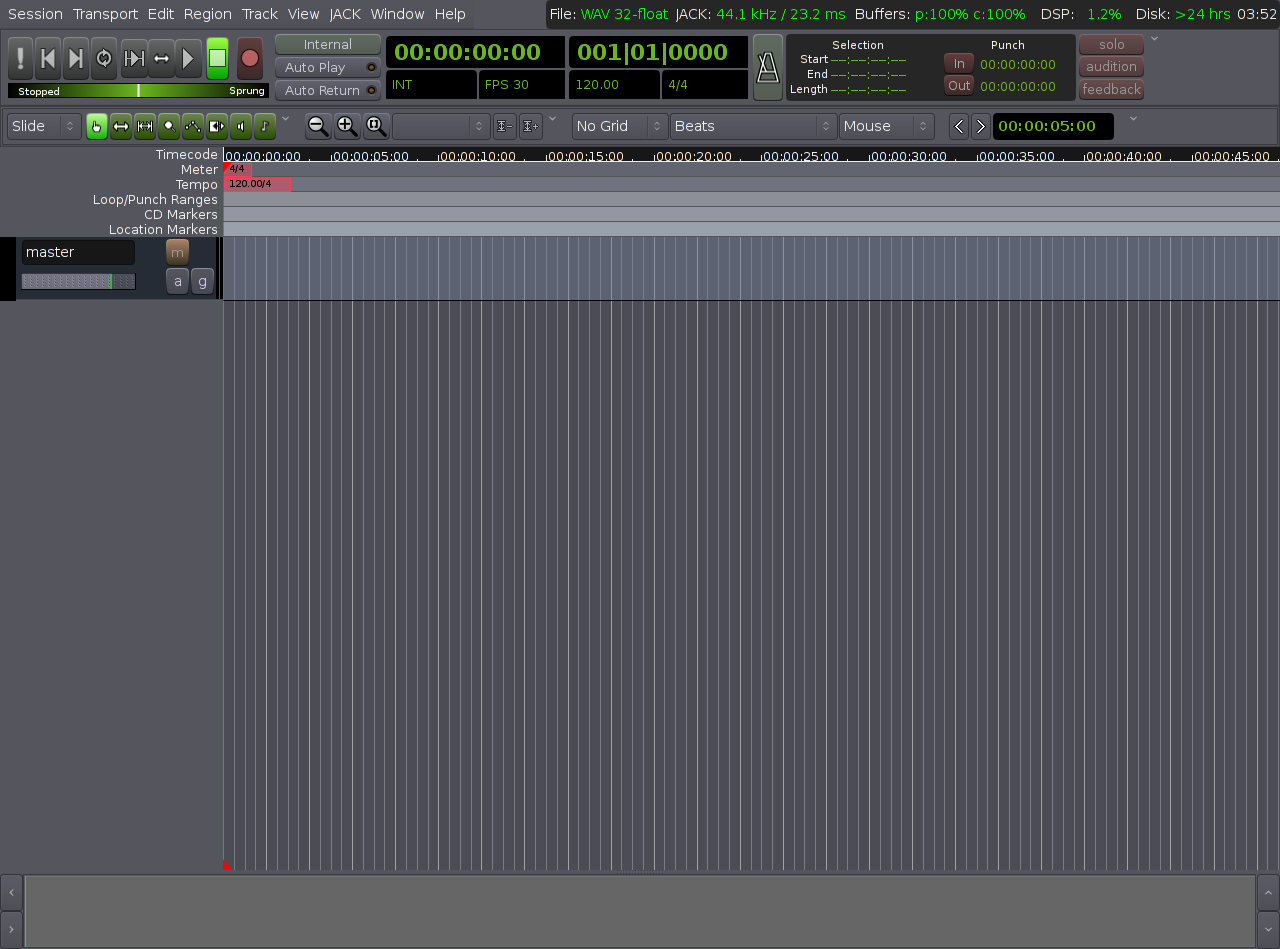
\includegraphics[scale=0.3]{screenshots/editor.png}
\caption{\ldots and finally: the editor!}
\label{fig:editor}
\end{figure}

\section{Adding a track and connecting it up}

The next step is to add a track to our session so that we have
something to record onto.  Choose \menu{Track,Add Track or Bus...}
from the menu at the top of the editor window.  This will bring up a
dialogue box, as shown in Figure~\ref{fig:add-track-or-bus}.

\screenshot{add-track-or-bus.png}{Add Track or Bus dialogue}{fig:add-track-or-bus}

For now, leave the options as they are; this will create a single
monophonic audio track.  This track must now be connected to the sound
card so that it can record incoming audio.

\section{Recording}

\section{Adding another track as an overdub}

\section{Mix-down}

\section{Export}



\end{document}



